% Copyright (C) 2012-2016  Dmitry V. Levin <ldv@altlinux.org>
% Copyright (C) 2016  Elvira~Khabirova <lineprinter0@gmail.com>
% Permission is granted to copy, distribute and/or modify this document
% under the terms of the GNU Free Documentation License, Version 1.2
% or any later version published by the Free Software Foundation;
% with no Invariant Sections, no Front-Cover Texts, and no Back-Cover Texts.

\documentclass[pdf]{beamer}
\beamertemplatenavigationsymbolsempty
\usetheme{Warsaw}
\setbeamertemplate{headline}{}
\setbeamertemplate{footline}{}
\usepackage[utf8]{inputenc}
\usepackage[english,russian]{babel}
\usepackage{graphicx}
\usepackage{changepage}

\title{\Huge strace \\ structured output}
\author{\huge student: Elvira~Khabirova \\ mentor: Dmitry~Levin}
\date{GSoC 2016}

\logo{
\includegraphics[height=0.5cm]{basealt.jpg}}

\begin{document}

\begin{frame}
\titlepage
\end{frame}

\begin{frame}[fragile]{What is strace?}
\begin{itemize}
	\item A diagnostic, debugging and instructional userspace
	utility for Linux.

	\item It is used to monitor interactions between processes and
	the Linux kernel, which include system calls, signal
	deliveries, and changes of process state.

	\item CLI and multiple filtering capabilities make it a powerful
	yet easy to use tracing tool.

	\item Traditional (since 1991) strace output is C-like human readable.
\end{itemize}

{
\scriptsize
\begin{block}{\large sample output}
\begin{verbatim}
$ strace -s 0 -P /dev/urandom python3 < /dev/null
open("/dev/urandom", O_RDONLY|O_CLOEXEC) = 3
fcntl(3, F_GETFD)                       = 0x1 (flags FD_CLOEXEC)
read(3, ""..., 24)                      = 24
close(3)                                = 0
+++ exited with 0 +++
\end{verbatim}
\end{block}
}

\begin{itemize}
	\item The main strace GSoC project this year was to implement structured output for strace.
\end{itemize}
\end{frame}

\begin{frame}[fragile]{strace: traditional output}
\begin{adjustwidth}{-1em}{-1em}
    \tiny
\begin{verbatim}
$ strace cat
execve("/bin/cat", ["cat"], [/* 42 vars */]) = 0
brk(NULL)                               = 0x60d000
mmap(NULL, 4096, PROT_READ|PROT_WRITE, MAP_PRIVATE|MAP_ANONYMOUS, -1, 0) = 0x7f942b45a000
access("/etc/ld.so.preload", R_OK)      = -1 ENOENT (No such file or directory)
open("/etc/ld.so.cache", O_RDONLY|O_CLOEXEC) = 3
fstat(3, {st_mode=S_IFREG|0644, st_size=13164, ...}) = 0
mmap(NULL, 13164, PROT_READ, MAP_PRIVATE, 3, 0) = 0x7f942b448000
close(3)                                = 0
open("/lib64/libc.so.6", O_RDONLY|O_CLOEXEC) = 3
read(3, "\177ELF\2\1\1\3\0\0\0\0\0\0\0\0\3\0>\0\1\0\0\0\20\t\2\0\0\0\0\0"..., 832) = 832
fstat(3, {st_mode=S_IFREG|0755, st_size=1705640, ...}) = 0
mmap(NULL, 3811712, PROT_READ|PROT_EXEC, MAP_PRIVATE|MAP_DENYWRITE, 3, 0) = 0x7f942ae88000
mprotect(0x7f942b021000, 2097152, PROT_NONE) = 0
mmap(0x7f942b221000, 24576, PROT_READ|PROT_WRITE, MAP_PRIVATE|MAP_FIXED|MAP_DENYWRITE, 3, 0x199000) = 0x7f942b221000
mmap(0x7f942b227000, 14720, PROT_READ|PROT_WRITE, MAP_PRIVATE|MAP_FIXED|MAP_ANONYMOUS, -1, 0) = 0x7f942b227000
close(3)                                = 0
mmap(NULL, 4096, PROT_READ|PROT_WRITE, MAP_PRIVATE|MAP_ANONYMOUS, -1, 0) = 0x7f942b459000
mmap(NULL, 4096, PROT_READ|PROT_WRITE, MAP_PRIVATE|MAP_ANONYMOUS, -1, 0) = 0x7f942b458000
mmap(NULL, 4096, PROT_READ|PROT_WRITE, MAP_PRIVATE|MAP_ANONYMOUS, -1, 0) = 0x7f942b457000
arch_prctl(ARCH_SET_FS, 0x7f942b458700) = 0
mprotect(0x7f942b221000, 16384, PROT_READ) = 0
mprotect(0x60b000, 4096, PROT_READ)     = 0
mprotect(0x7f942b453000, 4096, PROT_READ) = 0
munmap(0x7f942b448000, 13164)           = 0
brk(NULL)                               = 0x60d000
brk(0x62e000)                           = 0x62e000
brk(NULL)                               = 0x62e000
fstat(1, {st_mode=S_IFCHR|0620, st_rdev=makedev(136, 2), ...}) = 0
fstat(0, {st_mode=S_IFCHR|0666, st_rdev=makedev(1, 3), ...}) = 0
fadvise64(0, 0, 0, POSIX_FADV_SEQUENTIAL) = 0
mmap(NULL, 139264, PROT_READ|PROT_WRITE, MAP_PRIVATE|MAP_ANONYMOUS, -1, 0) = 0x7f942b431000
read(0, "", 131072)                     = 0
munmap(0x7f942b431000, 139264)          = 0
close(0)                                = 0
close(1)                                = 0
close(2)                                = 0
exit_group(0)                           = ?
+++ exited with 0 +++
\end{verbatim}
\end{adjustwidth}
\end{frame}

\begin{frame}[fragile]{strace: traditional output}
\begin{adjustwidth}{-1em}{-1em}
\begin{scriptsize}
\begin{verbatim}

$ strace -etrace=pwritev -ewrite=1 -s2 ./preadv-pwritev
...
pwritev(1, [{iov_base="01"..., iov_len=3}, {iov_base="34"..., iov_len=5}, ...],
3, 0) = 15
 * 3 bytes in buffer 0
 | 00000  30 31 32                                          012              |
 * 5 bytes in buffer 1
 | 00000  33 34 35 36 37                                    34567            |
 * 7 bytes in buffer 2
 | 00000  38 39 61 62 63 64 65                              89abcde          |
\end{verbatim}
\end{scriptsize}
\end{adjustwidth}
\note{Вывод дампа данных}
\end{frame}

\begin{frame}[fragile]{strace: traditional output}
\begin{scriptsize}
\begin{verbatim}

$ strace -c sync
% time     seconds  usecs/call     calls    errors syscall
------ ----------- ----------- --------- --------- ----------------
100.00    0.012000       12000         1           sync
  0.00    0.000000           0         1           read
  0.00    0.000000           0         3           open
  0.00    0.000000           0         5           close
  0.00    0.000000           0         3           fstat
  0.00    0.000000           0         7           mmap
  0.00    0.000000           0         4           mprotect
  0.00    0.000000           0         1           munmap
  0.00    0.000000           0         3           brk
  0.00    0.000000           0         3         3 access
  0.00    0.000000           0         1           execve
  0.00    0.000000           0         1           arch_prctl
------ ----------- ----------- --------- --------- ----------------
100.00    0.012000                    33         3 total

\end{verbatim}
\end{scriptsize}
\end{frame}


\begin{frame}[fragile]{parsers of traditional output: pystrace}
\begin{tiny}
\begin{verbatim}
global re_extract_unfinished
re_extract_unfinished \
		= re.compile(r"\s*(\d+\.\d+ .*) <unfinished \.\.\.>$")

global re_extract_resumed
re_extract_resumed \
		= re.compile(r"\s*(\d+\.\d+) <\.\.\. [\a-zA-Z\d]+ resumed>(.*)$")

global re_extract_signal
re_extract_signal \
		= re.compile(r"\s*(\d+\.\d+) --- (\w+) \(([\w ]+)\) @ (\d)+ \((\d+)\) ---$")

global re_extract_arguments_and_return_value_none
re_extract_arguments_and_return_value_none \
		= re.compile(r"\((.*)\)[ \t]*= (\?)$")

global re_extract_arguments_and_return_value_ok
re_extract_arguments_and_return_value_ok \
		= re.compile(r"\((.*)\)[ \t]*= (-?\d+)$")

global re_extract_arguments_and_return_value_ok_hex
re_extract_arguments_and_return_value_ok_hex \
		= re.compile(r"\((.*)\)[ \t]*= (-?0[xX][a-fA-F\d]+)$")

global re_extract_arguments_and_return_value_error
re_extract_arguments_and_return_value_error \
		= re.compile(r"\((.*)\)[ \t]*= (-?\d+) (\w+) \([\w ]+\)$")

global re_extract_arguments_and_return_value_error_unknown
re_extract_arguments_and_return_value_error_unknown \
		= re.compile(r"\((.*)\)[ \t]*= (\?) (\w+) \([\w ]+\)$")

global re_extract_arguments_and_return_value_ext
re_extract_arguments_and_return_value_ext \
		= re.compile(r"\((.*)\)[ \t]*= (-?\d+) \(([^()]+)\)$")

global re_extract_arguments_and_return_value_ext_hex
re_extract_arguments_and_return_value_ext_hex \
		= re.compile(r"\((.*)\)[ \t]*= (-?0[xX][a-fA-F\d]+) \(([^()]+)\)$")
\end{verbatim}
\end{tiny}
\end{frame}

\begin{frame}[fragile]{parsers of traditional output: buildreq}
\begin{adjustwidth}{-1.2em}{-1.2em}
\begin{scriptsize}
\begin{verbatim}
#!/bin/awk -f
# [...]
/^[1-9][0-9]*[[:space:]]+.* <unfinished \.\.\.>$/ {
    pid = $1;
    sub(" <unfinished \\.\\.\\.>$", "");
    trace[pid] = $0;
    next;
}

/^[1-9][0-9]*[[:space:]]+<\.\.\. [[:alnum:]_]+ resumed>/ {
    pid = $1;
    if (trace[pid] != "")
        sub("^[1-9][0-9]*[[:space:]]+<\\.\\.\\. [[:alnum:]_]+ resumed>", trace[pid]);
}

match($0, /^[1-9][0-9]*[[:space:]]+([[:alnum:]_]+at)\([^",]+, "(\/[^"]*)", .*\) += [[:alnum:]]+$/, ary) {
    delete trace[$1];
    output(ary[1], ary[2]);
    next;
}

match($0, /^[1-9][0-9]*[[:space:]]+([[:alnum:]_]+)\("(\/[^"]*)", .*\) += [[:alnum:]]+$/, ary) {
    delete trace[$1];
    output(ary[1], ary[2]);
    next;
}

/^[1-9][0-9]*[[:space:]]+/ { delete trace[$1]; }
\end{verbatim}
\end{scriptsize}
\end{adjustwidth}
\end{frame}


\begin{frame}{strace: converted code to produce structured output}
\begin{figure}[h]
      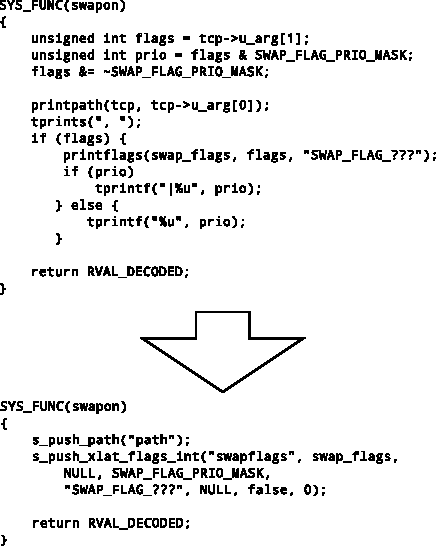
\includegraphics[width=0.6\textwidth]{lp0-conversion}
\end{figure}
\end{frame}

\begin{frame}{strace: structured output}
\begin{figure}[h]
      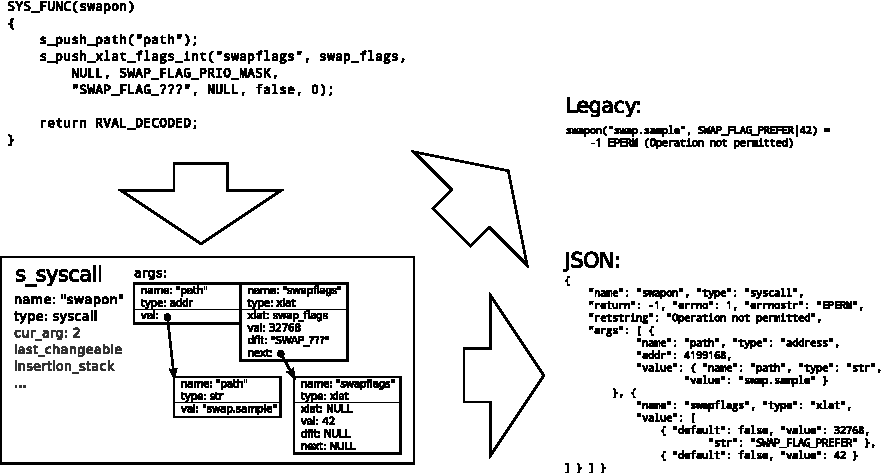
\includegraphics[width=\textwidth]{lp0-structured}
\end{figure}
\end{frame}

\begin{frame}{structured output: benefits for strace users}
\begin{itemize}
\item Less code redundancy, less bugs!
\item Easy to write robust parsers of strace output.
\item Secret \texttt{-z} option works for the first time.
\item Names of syscall arguments are available, both for traditional and structured output.
\end{itemize}
\end{frame}

\end{document}
